\documentclass[CJK, 8pt]{beamer}
\usepackage{CJKutf8}
\usepackage{graphicx}
\usetheme{Copenhagen}
%\usetheme{Boadilla}
\setbeamercovered{transparent}

\usepackage[T1]{fontenc}
\usepackage[default]{gillius}

\begin{document}

\begin{CJK*}{UTF8}{gkai}

\title{Leveldb原理与源码剖析}
\author{youngsterxyf}
\date{2014.08.31}

\begin{frame}[plain]
	\titlepage
\end{frame}

\section{简介}
\begin{frame}{Leveldb简介}
\begin{block}{特点}
	\begin{itemize}
	\item 持久化存储的KV系统
	\item 记录按Key有序存储
	\item 应用场景:写远远多于读
	\item LIB, NO SERVER --- 好处是?
	\item 单进程
	\end{itemize}
\end{block}

\begin{block}{测评}
	\begin{itemize}	
	\item 随机写:40万条记录每秒
	\item 随机读:6万条记录每秒
	\item 顺序读?
	\end{itemize}
\end{block}
\end{frame}

\begin{frame}{应用案例}
\begin{block}{}
	\begin{itemize}
	\item InfluxDB
	\item BigTable
	\item Google Chrome IndexDB
	\item 淘宝Tair的持久化存储引擎
	\item 可作为很多存储方案的存储引擎(如cayley、Riak)
	\item 异步消息队列的Broker
	\end{itemize}
\end{block}
\end{frame}

\section{基本原理}
\begin{frame}{Leveldb基本原理}
\begin{center}
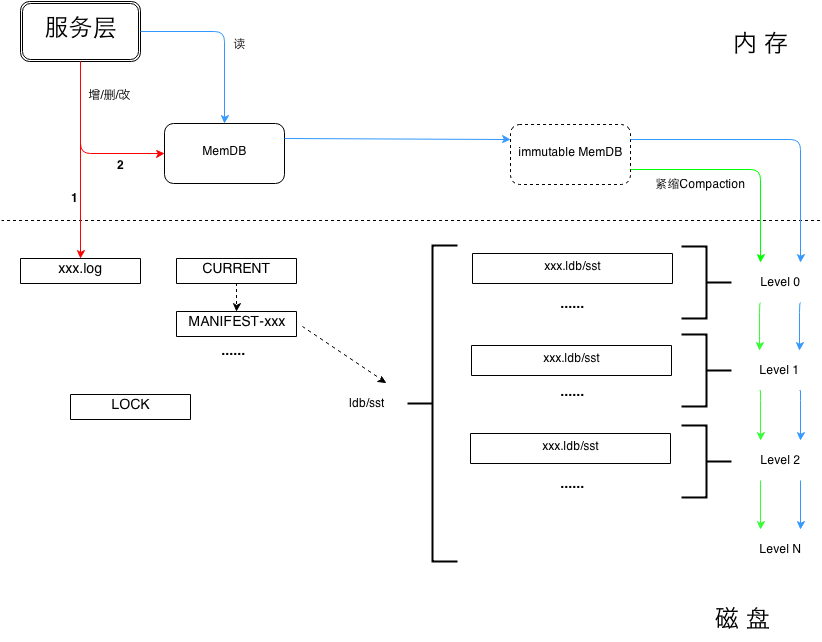
\includegraphics[height=6.5cm]{leveldb-arch-diagram.png}
\end{center}
\end{frame}

\section{简单实践}
\begin{frame}{LevelDB的使用}
\begin{block}{}
如何使用LevelDB?程序演示... {\color{blue}\href{https://github.com/HappyTechGroup/1st-phase/tree/master/leveldb/code}{源码见Github}}

逐个接口探索实现...
\end{block}
\end{frame}

\section{关键源码剖析}

\subsection{初始化}
\begin{frame}{基本逻辑}
初始化的过程就是打开数据库的过程-
\begin{enumerate}
\item 首先初始化一些数据结构,如d.tableCache、d.mem
\item 然后尝试创建数据存储目录,并创建LOCK文件,加文件锁。
\item 如果不存在CURRENT文件,则说明应该是首次打开数据库,需要创建manifest文件,并向文件中写入用户key比较方法的名称以及下一个可用的文件序号,然后创建CURRENT文件,在其中写入新manifest文件的文件名。
\item 接着,不管是否是首次打开数据库,都要先读取CURRENT文件内容,继而读取CURRENTS所指向的manifest文件的内容,对于其中的每条记录解析得到comparatorName、logNumber、nextFileNumber、lastSequence、compactPointer、\\deletedFiles、newFiles、preLogNumber(不一定都有),根据deleteFiles、newFiles计算出每个level持有的文件列表
\item 根据前一步骤得到的数据生成一个version(并且会计算该version的compactionScore和compactionLevel),放入d.versions链表中
\item 然后读取原来记录写入mem的操作的日志文件,根据日志内容重做其中的操作,存入一个临时的memtable中,然后转存入磁盘的level0 db文件中
\item 然后创建新的日志文件,设置d.log、d.logFile,并根据前一步骤重做日志产生的versionEdit和d.versions.currentVersion()生成一个新的version添加到d.versions上,并将versionEdit的内容写入manifest文件
\item 删除多余的文件(老log文件、当前version不需要的db文件等)
\item 尝试发起compaction(compaction的具体细节见“紧缩”一节)
\end{enumerate}
\end{frame}
\subsection{插入/更新}
\begin{frame}{基本逻辑}
对于Leveldb来说,插入/更新是同一个操作SET,过程如下:
\begin{enumerate}
\item 先将SET操作的key、value封装进一个batch,然后将batch的数据存储到d.mem所指的内存空间中,在存入d.mem之前需要检测d.mem是否还有剩余可用空间
\item 若没有,则将d.imm指向原来d.mem指向的内容空间,为d.mem申请一块新的内容空间,并创建新log文件设置d.logNumber、d.log、d.logFile,然后尝试发起compaction
\item 在存入d.mem之前还需要先把数据(batch.data)写入log文件并持久化。
\item 最后从batch中逐个读取kind、ukey、value,根据ukey生成内部key,然后以内部key为key想d.mem中写入value
\end{enumerate}
\end{frame}

\subsection{删除}
\begin{frame}{基本逻辑}
删除操作(DELETE)的过程与插入/更新的过程基本一致。因为Leveldb并不会真的去删除key、value对。
DELETE操作,用户只提供了key,在封装成batch时,仅将key封装进去,同时将操作类型(internalKeyKindDelete=0)也封装进去。
\end{frame}

\subsection{紧缩}
\begin{frame}{基本逻辑}
由前述内容可知,在初始化或SET操作d.mem已写满时,可能会有compaction过程。

\begin{block}{}
\begin{itemize}
\item compaction是否发起,和d.imm是否为nil以及d.versions.currentVersion().compaction\\Score是否大于1有关
\item 实际的compaction过程是在一个新的goroutine中执行的
\end{itemize}
\end{block}
\end{frame}
\begin{frame}{基本逻辑(续)}
当d.imm不为nil时,
\begin{enumerate}
\item 先将d.imm中的数据转存入level0的一个新的db文件中,转存的过程就是从d.imm逐项读出数据写入该新db文件中,然后返回该新db文件的元信息(fileNum、small\\est、largest、size)
\item 接着根据上一步返回的元信息封装一个versionEdit,与d.versions.currentVersion()生成一个新的version,并计算该version的compactionScore和compactionLevel,计算方法为:
	\begin{enumerate}
	\item 对于level0,计算$float64(len(v.files[0])) / l0CompactionTrigger$
	\item 对于非0 level,计算$float64(totalSize(v.files[level])) / maxBytes$,maxBytes初始为$float64(10 * 1024 * 1024)$,然后level每增大1,maxBytes则增大10倍
	\item 从1和2中找出最大的一个值作为version的compactionScore,这个最大的值对应的level作为version的compactionLevel
	\end{enumerate}
\item 将versionEdit信息写入manifest文件中
\end{enumerate}
\end{frame}
\begin{frame}{基本逻辑(续)}
除了d.imm不为nil时,需要将d.imm compaction到level0外,紧缩过程都是根据当前version的compactionLevel(假设为level n)(若$compactionScore >= 1$)
\begin{enumerate}
\item 先从level n、level n+1、level n+2找出内部key范围有重合的所有文件
\item 然后将这些文件的内容写到一个新的db文件中,并将该新db文件加到level n+1持有的文件列表中,从level n和level n+1持有的文件列表中删除找出来的文件(咦,level n+2呢?),从而得到一个新的versionEdit
\item 将新得到的versionEdit与当前的version合并生成一个新的version,放到d.versions中
\item 真正删除无用的db文件、log文件等
\item 在完成一次compaction后,由于某个level的文件数和文件内容大小有所变化,也生成了新的version、新的compactionScore和compactionLevel,所以会再次尝试发起compaction
\end{enumerate}
\end{frame}
\subsection{查找}
\begin{frame}{基本逻辑}
\begin{block}{查找流程}
\begin{enumerate}
\item 根据用户提供的key,封装成内部key
\item 根据内部key,依次从d.mem、d.imm中查找
\item 第2步若没有找到,则接着依次从level 0、level 1、...中查找
\end{enumerate}
\end{block}
\begin{block}{}
\begin{itemize}
\item 由于level 0和其他非0 level的db文件组织方式不相同,所以查找的方式也不一样
\item 为什么查找的顺序依次为d.mem、d.imm、level 0、level 1、...呢?
\end{itemize}
\end{block}
\end{frame}

\section{参考资料}
\begin{frame}{参考资料}
\begin{itemize}
{\color{blue}
\item \href{http://www.cnblogs.com/haippy/archive/2011/12/04/2276064.html}{数据分析与处理之二(Leveldb 实现原理)}
\item \href{http://leveldb.googlecode.com/svn/trunk/doc/index.html}{Leveldb官方文档}
\item \href{https://code.google.com/p/leveldb/}{Leveldb - Google Code}
\item \href{http://dirlt.com/leveldb.html}{Leveldb - dirlt.com}
}
\end{itemize}
\end{frame}

\begin{frame}{Q \& A}
\begin{center}
谢 谢!
\end{center}
\end{frame}
\end{CJK*}
\end{document}